\documentclass{amsmlaj}

\begin{document}
\lecturesol{Homework 3}{Ke Tran}{m.k.tran@uva.nl}{April 26, 2016}
{Andrea Jemmett}{11162929}{andreajemmett@gmail.com}{N/A}

\begin{problem}
Consider the inference problem of evaluating $p(\vt{x}_n|\vt{x}_N)$ for the
graph shown in Figure \ref{fig:chain}, for all nodes $n \in \{1,\dotsc,N-1\}$.
Show that the message passing algorithm can be used to solve this efficiently,
and discuss which messages are modified and in what way.

\begin{figure}[H]
\begin{center}
\begin{tikzpicture}
\node[nObs,] (x1) at (0,0) {};
\node at (0,-0.5) {$x_1$};
\node[nObs,] (xn_1) at (3,0) {};
\node at (3,-0.5) {$x_{n-1}$};
\node[nObs,] (xn) at (4.5,0) {};
\node[nObs,] (xn1) at (6,0) {};
\node at (6,-0.5) {$x_{n+1}$};
\node at (4.5,-0.5) {$x_n$};
\draw [-, thick, red] (x1) -- (1,0);
\draw[dashed, thick, red] (1,0) -- (2,0);
\draw [-, thick, red]  (2,0) -- (xn_1);
\draw [-, thick, red]  (xn_1) -- (xn);
\draw [-, thick, red]  (xn) -- (xn1);
\draw [-, thick, red]  (xn1) -- (7,0);
\draw[dashed, thick, red] (7,0) -- (8,0);
\node[nObs,] (xN) at (9,0) {};
\node at (9,-0.5) {$x_N$};
\draw [-, thick, red] (8,0) -- (xN);
% draw messages
\node at (2,0.7) {$\mu_\alpha(x_{n-1})$};
\draw [->, thick, blue] (2,0.4) -- (2.5,0.4);
\node at (3.75,0.7) {$\mu_\alpha(x_n)$};
\draw [->, thick, blue] (3.5,0.4) -- (4,0.4);
\node at (5.25,0.7) {$\mu_\beta(x_n)$};
\node at (7,0.7) {$\mu_\beta(x_{n+1})$};
\draw [->, thick, blue] (5.5,0.4) -- (5,0.4);
\draw [->, thick, blue] (7,0.4) -- (6.5,0.4);
\end{tikzpicture}
\caption{Chain of nodes model}
\label{fig:chain}
\end{center}
\end{figure}
\end{problem}

\begin{problem}
Apply the sum-product algorithm to the chain of nodes model in Figure
\ref{fig:chain}  and show that the results of message passing algorithm are
recovered as a special case, that is
\begin{eqnarray}
p(x_n) & = & \frac{1}{Z}\mu_\alpha(x_n)\mu_\beta(x_n) \nonumber\\
\mu_\alpha(x_n) & = & \sum\limits_{x_n-1} \psi_{n-1,n}(x_{n-1},x_n)\mu_\alpha(x_{n-1}) \nonumber\\
\mu_\beta(x_n) & = & \sum\limits_{x_{n+1}} \psi_{n+1,n}(x_{n+1},x_n)\mu_\beta(x_{n+1}) \nonumber
\end{eqnarray}
where $\psi_{i,i+1}(x_i,x_{i+1})$ is a potential function defined over clique $\{x_i,x_{i+1}\}$.

\begin{sol}
	\begin{figure}[h]
		\centering
		\begin{tikzpicture}
			\node[nObs, red] (x1) at (0,0) {};
			\node at (0,.5) {$x_1$};
			\node[fact] (f12) at (1.5,0) {};
			\node at (1.5,-.5) {$\psi_{1,2}(x_1,x_2)$};
			\draw[-, red] (x1) -- (f12);
			\node[nObs,red] (x2) at (3,0) {};
			\node at (3,.5) {$x_2$};
			\node[fact] (f23) at (4.5,0) {};
			\node at (4.5,-.5) {$\psi_{2,3}(x_2,x_3)$};
			\draw[-, red] (f12) -- (x2);
			\draw[-, red] (x2) -- (f23);
			\node[nObs, red] (xn_1) at (6,0) {};
			\node at (6,.5) {$x_{n-1}$};
			\draw[-, red] (f23) -- (5,0);
			\draw[dashed, red] (5,0) -- (5.5,0);
			\draw[-, red] (5.5,0) -- (xn_1);
			\node[fact] (fn_1n) at (7.5,0) {};
			\node at (7.5,-.5) {$\psi_{n-1,n}(x_{n-1},x_n)$};
			\draw[-, red] (xn_1) -- (fn_1n);
			\node[nObs, red] (xn) at (9,0) {};
			\node at (9,.5) {$x_n$};
			\draw[-, red] (fn_1n) -- (xn);
			\node[fact] (fnn1) at (10.5,0) {};
			\node at (10.5,-.5) {$\psi_{n,n+1}(x_n,x_{n+1})$};
			\draw[-, red] (xn) -- (fnn1);
			\node[nObs, red] (xn1) at (12,0) {};
			\node at (12,.5) {$x_{n+1}$};
			\draw[-, red] (fnn1) -- (xn1);
			\node[fact] (fN) at (13.5,0) {};
			\node at (13.5, -.5) {$\psi_{N-1,N}(x_{N-1},x_N)$};
			\draw[-, red] (xn1) -- (12.5,0);
			\draw[dashed, red] (12.5,0) -- (13,0);
			\draw[-, red] (13,0) -- (fN);
			\node[nObs, red] (xN) at (15,0) {};
			\node at (15,.5) {$x_N$};
			\draw[-, red] (fN) -- (xN);
		\end{tikzpicture}
		\caption{Factor graph for chain of nodes model}
		\label{fig:chain-factor}
	\end{figure}

	The first thing to do to apply the sum-product algorithm to the chain model of
	Figure \ref{fig:chain} is to transform it into a factor graph. The factor
	graph for the chain model is shown in Figure \ref{fig:chain-factor}.

	Once we have a factor graph, we need to chose a root node, \eg $x_n$, so that
	we can start propagating messages from the leaf nodes ($x_1$ and $x_N$) to the
	root. We start by propagating messages from $x_1$ to the root:
	\begin{align}
		\mu_{x_1 \to \psi_{1,2}}(x_1)&=1\\
		\mu_{\psi_{1,2} \to x_2}(x_2)&=\sum_{x_1}\psi_{1,2}(x_1,x_2)\\
		\mu_{x_2 \to \psi_{2,3}}(x_2)&=\mu_{\psi_{1,2} \to x_2}(x_2)\\
		\mu_{\psi_{2,3} \to x_3}(x_3)
			&=\sum_{x_2}\psi_{2,3}(x_2,x_3)\mu_{x_2 \to \psi_{2,3}}(x_2)\\
		\vdots\qquad&\qquad\vdots \nonumber \\
		\mu_{x_{n-1} \to \psi_{n-1,n}}(x_{n-1})
			&=\mu_{\psi_{n-2,n-1} \to x_{n-1}}(x_{n-1}) \\
		\mu_{\psi_{n-1,n} \to x_n}(x_n)
			&=\sum_{x_{n-1}}\psi_{n-1,n}(x_{n-1},x_n)\mu_{x_{n-1} \to \psi_{n-1,n}}(x_{n-1})
	\end{align}
	and we note that a message that a variable node sends on one link is equal to
	the message that node has received on its other link. That is variable nodes
	act as \textit{proxies} for messages created at factor nodes.

	If we define $\mu_\alpha(x_n)$ as the incoming from the left factor node to
	variable node $x_n$, we have that
	\begin{align}
		\mu_\alpha(x_n)
		&\equiv\mu_{\psi_{n-1,n} \to x_n}(x_n) \\
		&=\sum_{x_{n-1}}\psi_{n-1,n}(x_{n-1},x_n)\mu_{x_{n-1} \to \psi_{n-1,n}}(x_{n-1}) \\
		&=\sum_{x_{n-1}}\psi_{n-1,n}(x_{n-1},x_n)\mu_{\psi_{n-2,n-1} \to x_{n-1}}(x_{n-1}) \\
		&=\sum_{x_{n-1}}\psi_{n-1,n}(x_{n-1},x_n)\mu_\alpha(x_{n-1})
	\end{align}

	If we compute in the same way the messages from leaf node $x_N$ to the root
	node $x_n$, we obtain that
	\begin{align}
		\mu_\beta(x_n)
		&\equiv \mu_{\psi_{n,n+1} \to x_n}(x_n) \\
		&=\sum_{x_{n+1}} \psi_{n,n+1}(x_n,x_{n+1})\mu_{x_{n+1} \to \psi_{n,n+1}} \\
		&=\sum_{x_{n+1}}\psi_{n,n+1}(x_n,x_{n+1})\mu_{\psi_{n+1,n+2} \to x_{n+1}}(x_{n+1}) \\
		&=\sum_{x_{n+1}}\psi_{n,n+1}(x_n,x_{n+1})\mu_\beta(x_{n+1})
	\end{align}

	Finally applying eq. 8.63 from Bishop (with the addition of the normalizing
	constant $Z$ that we know from the full joint distribution or we can compute
	locally on the node $x_n$) we have that
	\begin{align}
		p(x_n)
		&=\frac{1}{Z}\mu_{\psi_{n-1,n} \to x_n}(x_n) \mu_{\psi_{n,n+1} \to x_n}(x_n) \\
		&=\frac{1}{Z}\mu_\alpha(x_n) \mu_\beta(x_n)
	\end{align}
\end{sol}

\end{problem}

\newpage

\begin{problem}
Run sum-product algorithm on the graph in Figure \ref{fig:simplegraph} with node
$x_3$ designed as the root. Using the computed messages given in \emph{p.409 Bishop}.
\begin{enumerate}
\item  Show that the correct marginals are obtained for $x_1$ and $x_3$.
\item Show that the sum-product algorithm on this graph gives the correct joint distribution for $x_1$, $x_2$.
\end{enumerate}

\begin{figure}[H]
\begin{center}
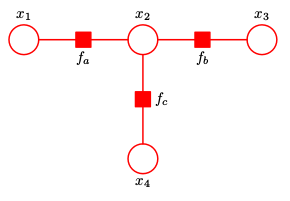
\includegraphics[width=.4\textwidth]{simplegraph.png}
\caption{A simple factor graph}
\label{fig:simplegraph}
\end{center}
\end{figure}

\begin{sol}
	\begin{enumerate}
		\item
			\begin{align}
				p(x_1)
				&=\mu_{f_a \to x_1}(x_1) \\
				&=\sum_{x_2} f_a(x_1,x_2) \mu_{x_2 \to f_a}(x_2) \\
				&=\sum_{x_2} f_a(x_1,x_2) \mu_{f_b \to x_2}(x_2) \mu_{f_c \to x_2}(x_2) \\
				&=\sum_{x_2} f_a(x_1,x_2) \sum_{x_3}f_b(x_2,x_3) \sum_{x_4}f_c(x_2,x_4) \\
				&=\sum_{x_2,x_3,x_4}f_a(x_1,x_2)f_b(x_2,x_3)f_c(x_2,x_4) \\
				&=\sum_{x_2,x_3,x_4}p(x_1,x_2,x_3,x_4)
			\end{align}
			\begin{align}
				p(x_3)
				&=\mu_{f_b \to x_3}(x_3) \\
				&=\sum_{x_2}f_b(x_2,x_3) \mu_{x_2 \to f_b}(x_2) \\
				&=\sum_{x_2}f_b(x_2,x_3) \mu_{f_a \to x_2}(x_2) \mu_{f_c \to x_2}(x_2) \\
				&=\sum_{x_2}f_b(x_2,x_3) \sum_{x_1}f_a(x_1,x_2) \sum_{x_4}f_c(x_2,x_4) \\
				&=\sum_{x_1, x_2, x_4} f_b(x_2,x_3) f_a(x_1,x_2) f_c(x_2,x_4) \\
				&=\sum_{x_1,x_2,x_4} p(x_1,x_2,x_3,x_4)
			\end{align}
		\item
			\begin{align}
				p(x_1,x_2)
				&=f_a(x_1,x_2) \mu_{x_1 \to f_a}(x_1) \mu_{x_2 \to f_a}(x_2) \\
				&=f_a(x_1,x_2) \mu_{f_b \to x_2}(x_2) \mu_{f_c \to x_2}(x_2) \\
				&=f_a(x_1,x_2) \sum_{x_3} f_b(x_2,x_3) \sum_{x_4} f_c(x_2,x_4) \\
				&=f_a(x_1,x_2) \sum_{x_3,x_4} f_b(x_2,x_3) f_c(x_2,x_4) \\
				&=\sum_{x_3,x_4} f_a(x_1,x_2) f_b(x_2,x_3) f_c(x_2,x_4) \\
				&=\sum_{x_3,x_4} p(x_1,x_2,x_3,x_4)
			\end{align}
	\end{enumerate}
\end{sol}

\end{problem}

\begin{problem}
Show that the marginal distribution for the variables $\vt{x}_s$ in a factor
$f_s(\vt{x}_s)$ in a tree-structured factor graph, after running the sum-product
message passing algorithm, can be written as
\[
p(\vt{x}_s) = f_s(\vt{x}_s) \prod\limits_{i \in \text{ne}(f_s)} \mu_{x_i \to f_s(x_i)}
\]
where ne($f_s$) denotes the set of variable nodes that are neighbors of the factor node $f_s$
\end{problem}

\end{document}

